% Modern editorial, markup and figure/layout contributions: CC-BY-SA-4.0.
% Historical text and illustrations: Leonhard Euler (1744), public domain.
% Component scope and upstream attribution: see RIGHTS.md.
% Manual vector redraw from E65 Tabula II, Fig. 13.
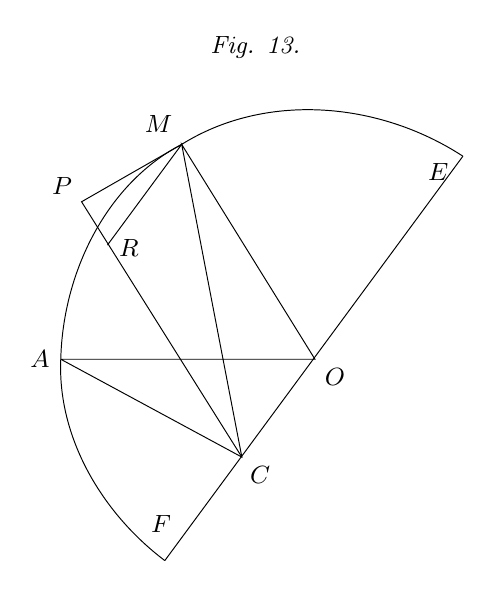
\begin{tikzpicture}[x=1cm,y=1cm,line width=.35pt,font=\small]
\draw (0.5286,2.7357)--(3.7571,2.7357)--(2.0643,5.4643)--(2.8286,1.4929)--(0.5286,2.7357);
\draw (1.8500,0.1786)--(5.6357,5.3143);
\draw (2.8286,1.4929)--(0.7929,4.7357)--(2.0643,5.4643)--(1.1214,4.1857);
\draw (1.8500,0.1786) .. controls (1.0571,0.7786) and (0.4857,1.7357) .. (0.5286,2.7357) .. controls (0.5571,3.8643) and (1.1286,4.9786) .. (2.0643,5.4643) .. controls (3.1143,6.1214) and (4.5500,6.0214) .. (5.6357,5.3143);
\node[anchor=east,inner sep=1pt] at (0.4286,2.7357) {$A$};
\node[anchor=south east,inner sep=1pt] at (1.9857,5.5714) {$M$};
\node[anchor=north east,inner sep=1pt] at (5.4929,5.2643) {$E$};
\node[anchor=north west,inner sep=1pt] at (3.8429,2.6643) {$O$};
\node[anchor=north west,inner sep=1pt] at (2.8929,1.4214) {$C$};
\node[anchor=south east,inner sep=1pt] at (1.9714,0.5000) {$F$};
\node[anchor=south east,inner sep=1pt] at (0.7143,4.7929) {$P$};
\node[anchor=west,inner sep=1pt] at (1.2286,4.1429) {$R$};
\node[anchor=south] at (3.0000,6.4286) {\textit{Fig. 13.}};
\end{tikzpicture}
